
{\chapter{Exploring the single-cell RNAseq analysis landscape in timeseries patient derived xenografts}

}
 \label{ch:Chapter5}
 \section{Motivation}

In spite of advanced technologies and treatment, triple negative breast cancer still facing the problems of tumor recurrence and drug resistance.
For any given difference between the types of drug resistance, for example, the expression of a particular gene, it is assumed that differences arise deterministically or probabilistically in the configuration of transcription factors regulating the genes in the tumors. Cancer cells in distinct cell- states often exhibit important differences in functional properties depending on the which genes are turned on and off resulting in sensitive or resistant phenotype.

The most challenging analysis is to differentiate whether the change in gene expression leading to change in cellular state is stochastic\cite{raj2008nature} and random or its deterministic to produce the same output under similar environment.
Cancer cells in distinct cell- states often exhibit important differences in functional properties depending on which genes are turned on and off resulting in sensitive  or resistant phenotype.
Previously it is shown that unique cells within a population can exhibit fluctuations in expression of a group of genes, that could predict distinct phenotypes \cite{shaffer2019memory}.

Although many studies have analyzed CNV and differential gene expression of distinct oncogenes and tumor suppressor genes in various cancers \cite{kuzyk2015mycn, budczies2016pan, kwak2015fibroblast} but there has been no precise study about the relationship between CNV and differential gene expression across a multiple tumor samples. It is unclear to what extent the expression level is affected by CNV.  Because of difficulty to analyse longitudinal patient's samples for single cell gene expression and lack of multiple longitudinal pre-clinical breast cancer models, these questions remains unexplored and how they relate to triple negative breast cancer heterogeneity, is limited.

Here we aimed to systematically investigate the specific relationship between copy number change and differential gene expression across timeseries TNBC PDX for which we have clonal copy number proportions already known frorm chapter 4. We set to explore timeseries three breast cancer patient derived xenografts (PDX) that were serially challenged for around 4-5 cycles with the drug until they started showing less response to the treatment.The aim is to measure the magnitude of fluctuations in gene expression from sensitive to resistant phenotype.
This study may help us better understand the correlation between CNV and differential gene expression and provide new insights into the mechanism of development and progression of cancer with potential biomarkers in triple negative breast cancer.

 \section{Synopsis}
 From the previous chapter we know that the population changes with the tumor growth from one passage to another with and without the drugs. We see the shifts in the clones and some clones get selected and others disappear.
For this chapter, to explore the cellular compositions and heterogeneity under diverse conditions, in breast cancer, we performed scRNAseq analysis on the same 3 patient derived xenograft timeseries tumors used as substrates in chapter 4. We acquired transcriptional signatures of 171,560 individual cells. Two libraries from CX-5461 treated samples were excluded from analysis as they didn't pass our QC threshold. Total of 145,858 individual cells were taken into further transcriptome analysis, including  52,256 cells from untreated tumors, 40,754 cells from cisplatin treated tumors, 31,269 cells from cisplatin drug holiday tumors, 8,558 cells from CX-5461 treated tumors and 13,021 cells from CX-5461 drug holiday tumors. The detail after filtering is summarized in  \textbf{\autoref{tab:nofcellsRNA}}.

%------------------------------------------------------------------------
% Please add the following required packages to your document preamble:
% \usepackage{graphicx}
\begin{table}[htbp]
 \centering
  \caption{Number of cells sequenced for transcriptome analysis}
{
\begin{tabular}{|l|l|l|}
\hline
Sample labels     & No. of cells sequenced for scRNA & Filtered \\
\hline
Total cells          & 145,858                          & 63,183\\
Untreated         & 52,256                           & 21,510    \\
Cisplatin-Rx      & 40,754                           & 19,095    \\
Cisplatin-holiday & 31,269                           & 15,158    \\
CX-5461-Rx        & 8,558                            & 4,047     \\
CX-5461-holiday   & 13,021                           & 3,373  \\  
\hline
\end{tabular}%
\label{tab:nofcellsRNA}
}
\end{table}
%------------------------------------------------------------------------

To pursue our analysis in single cell RNA space, first, we summarized the clonal identities from chapter 4 into sensitive and resistant. We assume that the clones that show fitness advantage under drug selection, in DLP+ level, are resistant because they were high abundance clones and the tumors started responding less, whereas the clones that are having high fitness coefficient in the absence of drug are sensitive because they could not survive under drug pressure. Briefly summarized in  \textbf{\autoref{tab:Listofresistantandsensitiveclones}}.
 
Next, by using clonealign \cite{campbell2019clonealign}, we were able to assign single cell RNAseq to clones and observed similar clonal proportion from RNA seq what we concluded in the DLP+ in chapter 4. 
We did dimentionality reduction embedding of the cells and revealed that the clones appear to be clustering together with minor exceptions. 

%------------------------------------------------------------------------   
 % Table generated by Excel2LaTeX from sheet 'Sheet1'
 \begin{table}[htbp]
   
   \centering
   \caption{List of resistant and sensitive clones across TNBC PDX}
     \begin{tabular}{|l|l|l|}
      \hline
     TNBC PDX & Resistant clone & Sensitive clone \\
     \hline
     SA609  & Clone R & Clone H \\
     SA1035 & Clone H & Clone E \\
     SA535-Cisplatin Rx & Clone S\_T & Clone J \\
     SA535-CX-5461 Rx & Clone U & Clone J \\    \hline
     \end{tabular}%
   \label{tab:Listofresistantandsensitiveclones}%
   
  
 \end{table}%
%------------------------------------------------------------------------

Next, we asked how much of the expression is accounted by the change in copy number and what proportion is independent. The global proportions of \textit{in cis} and \textit{in trans} in resistant versus sensitive clones were measured. Then we looked for the magnitude of difference of upregulated or down regulated genes by calculating differential expression of resistant and sensitive clones through volcano plots analysis. Lastly, we explored which pathways and individual genes are involved in resistant and sensitive clones across all timeseries PDX models. We identified some genes that were monotonically increasing or decreasing under continuous drug pressure in our models. We found few intersecting pathways that seems to be upregulated in all timeserries and some with 2-3. We have identified certain commom genes that are showing trends under the drug and could be further investigated as potential biomarkers of disease progression and tumor response.

%------------------------------------------------------------------------
\begin{figure}
\centering
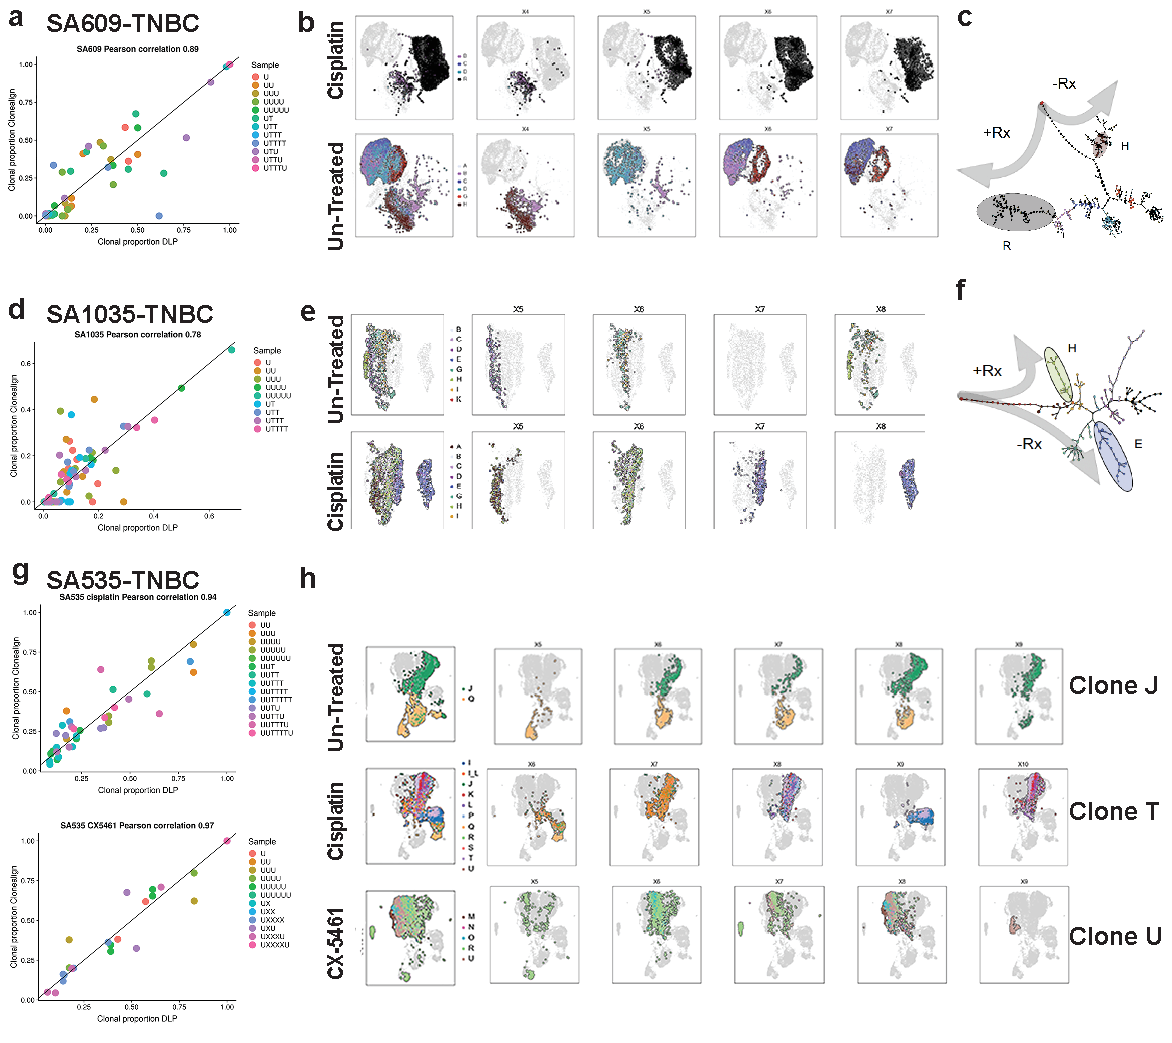
\includegraphics[width=\textwidth]{Figures/fig2_clonealignembeddings.pdf}
	
\caption[Gene expression impacts of clone-specific copy number profiles]
	{\small
	\textbf{Gene expression impacts of clone-specific copy number profiles.}
	   \textbf{(a)} \texttt{clonealign} clonal proportions vs DLP+ clonal proportions of SA609 PDX timeseries samples indicating positive correlation (Pearson correlation from 0.89).
	    \textbf{(b)} Low dimensional \ac{UMAP} embeddings of matching scRNAseq libraries across the SA609 TNBC timeseries. Left top and bottom panels show treated and untreated complete embedding annotated with clonealign assignments and right all panels show the density of cell clusters over the timeseries X4-X7.
	     \textbf{(c)} Phylogeny of SA609 taken from previous chapter to recall emerged clones with or without drug. 
	     \textbf{(d)} Same like \textbf{(a)} but for SA1035 PDX and Pearson correlation is 0.78. \textbf{(e)} Same like \textbf{(b)} but for SA1035 starting from X5-X8. \textbf{(f)} Same like \textbf{c} but for SA1035. \textbf{(g)} Same like \textbf{a} but for SA535 PDX and Pearson correlation is 0.94 for cisplatin treated and 0.97 with CX-5461 treated. \textbf{(h)} Same like \textbf{b} but for SA535 starting from X5-X9, X10.
	}
	\label{fig:fig2_clonealignembeddings.pdf}
\end{figure}

%------------------------------------------------------------------------

\section{Results}

\subsection{Clone-specific genotypes underpin clone-specific gene expression programs}
We profiled the impact of clone specific gene expression changes as a higher order representation of phenotypic properties. We tested if the genotypes of high fitness clones exhibited changes in their transcriptional program, with scRNAseq performed on matched aliquots of samples sequenced using DLP+ on the serially passaged triple-negative breast cancer patient-derived xenografts from Chapter 4 as substrates \textbf{\autoref{fig:treatedtimeseriesmanuscript}} and \textbf{\autoref{fig:SA535CX5461} a}.

\subsubsection{Copy number change and scRNAseq expression revealed high concordance across PDX timeseries}
  In our approach, we assume clones are defined through grouped cell subsets which share to a first approximation similar genomic copy number structure (e.g., through phylogenetic reconstruction or dimensionality reduction) \cite{laks2019clonal}. Based on this relationship we applied
  \texttt{clonealign}, a statistical method, \cite{campbell2019clonealign} to reveal clone-specific phenotypic properties across all samples.
  Each point is taken as the proportion of DLP cells in a clone horizontal axis versus the proportion of the scRNAseq cells in the same clone. The  correlation for all clones were then calculated by using Pearson correlation coefficient formula. The heat maps of SA609 TNBC PDX \textbf{(\autoref{fig:UnRxseries} h)} and SA535 TNBC PDX \textbf{(\autoref{fig:SA535analysis} a, e)} exhibit more complex heterogeneity at copy number space along with structural genomic rearrangements as compared to SA1035 TNBC PDX \textbf{(\autoref{fig:SA1035Rxnew} a, e)}. Our results showed DLP+ and \texttt{clonealign} clone abundance measures were positively correlated across all libraries \textbf{(\autoref{fig:fig2_clonealignembeddings.pdf} a, d, g)}. Importantly, SA535 TNBC treated with cisplatin presented the high confidence correlation with Pearson correlation 0.94 (p-value$< 10^{-18}$), followed by its CX-5461 treated series, presenting Pearson correlation of 0.97 (p-value$< 10^{-15}$) \textbf{\autoref{fig:fig2_clonealignembeddings.pdf} g}. However, SA609 PDX timeseries samples present a Pearson correlation coefficient of 0.89 (p-value $< 10^{-16}$) \textbf{(\autoref{fig:fig2_clonealignembeddings.pdf} a)} and SA1035 PDX with Pearson correlation of 0.78 (p-value$< 10^{-18}$) \textbf{(\autoref{fig:fig2_clonealignembeddings.pdf} d)}.
  
  
\subsubsection{Single cell RNAseq clusters exhibit relatively monomorphic pattern of global expression over time which tracked with clone assignments}
Having made the assignments of cells to clones, next, we visualized the data using UMAP \cite{becht2019dimensionality}, dimensionality reduction method, to aggregate cells into treated and untreated subpopulations while retaining the relationship between subpopulations. scRNAseq embeddings displayed a dynamic pattern of global expression over time with and without treatment, which tracked with clone assignments indicating co-variation of transcriptional properties with clonal abundance \textbf{\autoref{fig:fig2_clonealignembeddings.pdf}}. UMAP visualization of clusters identified clone H clusters in untreated setting and clone R clusters, in the cisplatin treated series of SA609 TNBC PDX, purified over time matching their genomically defined counterparts \textbf{(\autoref{fig:fig2_clonealignembeddings.pdf} b)}. Similarly, clone E in untreated and clone H in treated timeseries of SA1035  \textbf{(\autoref{fig:fig2_clonealignembeddings.pdf} e)}, clustered uniquely at the later time points. \textbf{\autoref{fig:fig2_clonealignembeddings.pdf} c, f} reminding the clones emerging with and without treatment through the phylogeny of DLP+ from chapter 4, in SA609 and SA1035, respectively.  SA535 TNBC PDX all three arms of untreated, treated with cisplatin and CX-5461, exhibited aggregation of similar patterns of clusters that favours emerging of genomic clones in their respective series. Clone J, in untreated control timeseries \textbf{(\autoref{fig:fig2_clonealignembeddings.pdf} h, upper panel)}, clone T, in cisplatin treated \textbf{(\autoref{fig:fig2_clonealignembeddings.pdf} h, middle panel)}, and clone U in CX-5461 treated \textbf{(\autoref{fig:fig2_clonealignembeddings.pdf} h, lower panel)}.

%------------------------------------------------------------------------

\begin{figure}
\centering
  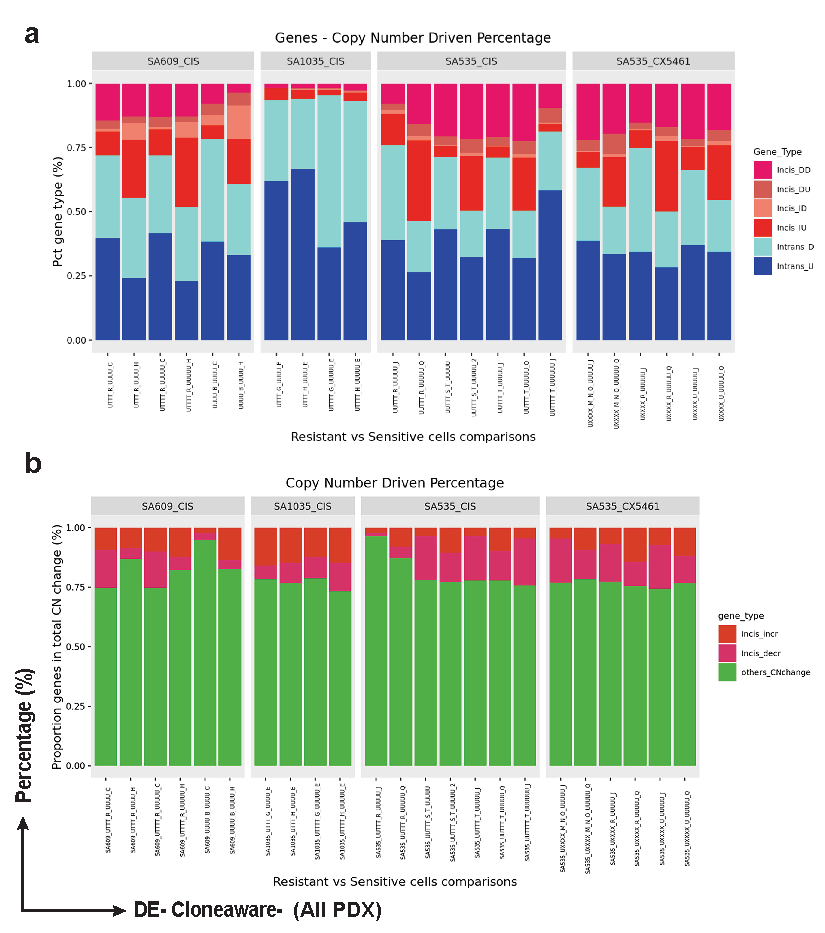
\includegraphics[width=\textwidth]{Figures/fig4Summaryincistrans.pdf}
	
\caption[Summary proportion of \textit{in cis} and \textit{in trans} regulated gene expression in scRNAseq data]
	{\small
	\textbf{Summary proportion of \textit{cis} and \textit{trans} regulated gene expression in scRNAseq data.}
	   Horizontal axis shows differential expression between two selected clones from all the three PDX treated and un-treated timeseries. Vertical axis gives percentages of genes.  \textbf{(a)}  Red and pink bars represent \textit{in cis} change in expression in both panels, and blue bars represent \textit{in trans} regulated gene expression.
	    \textbf{(a)} 
	    \textbf{(b)} 
	     
	}
	\label{fig:fig3Summaryincistrans}
\end{figure}

%---------------------------------------------------------------
\subsection{Quantitative single cell gene expression analysis unravels the rates of \textit{in cis} and \textit{in trans} components}

It is broadly acknowledged that somatic CNV is highly associated with the development and progression of numerous cancers by influencing gene expression level \cite{yang2017prame, gut2018sox2}. 
Here, we investigated as to how much of the proportions of \textit{in cis} and \textit{in trans} regulated genes in our procured single cell RNA expression data is influenced by the change in copy number.

To calculate the percentage of genes presenting \textit{in cis} or \textit{in trans} regulatory effects, the differential expression single cell RNAseq data was decomposed into \textit{cis}, where the gene expression that is following the change in copy number and \textit{trans}, where it is independent.

\subsubsection{Differential gene expression between resistant and sensitive clones exhibit high \textit{in trans} proportion.}

Firstly, we did differential expression analysis of resistant clones as in \textbf{\autoref{tab:Listofresistantandsensitiveclones}} and some of selected clones that were closely related to the resistant clones or having second highest fitness coefficients in DLP+ data from chapter 4, versus the sensitive ones from each of the time series PDX using \texttt{edgeR} \cite{robinson2010edger}. Then, we classified these genes into upregulated with increase in copy number (incis\_IU) and downregulated (incis\_DD) with decrease in copy number or upregulated with decrease in copy number (incis\_DU) or downregulated with increase in copy number (incis\_ID), from one clone to another, as mentioned in the legend of \textbf{\autoref{fig:fig3Summaryincistrans} a}.

From HMMcopy output of segment copy number position (chromosome start and end), we get gene coordinates by mapping our segment positions with reference database of known genes for human  \cite{carlson2015txdb}. First, we identify overlapping positions between chromosome segments and known genes, then we assigned those segments to an ensemble gene ID \cite{rainer2019ensembldb} of the  selected \ac{DE} of clones across all timeseries and calculated their number and percentages in each PDX timeseries  \textbf{\autoref{tab:DEpercentageincisintrans}}. Importantly, we found that the overall number of \textit{in trans} genes were higher as compared to \textit{in cis}, which is supporting previously reported results \cite{shao2019copy}. 


%------------------------------------------------------

% Please add the following required packages to your document preamble:
% \usepackage{graphicx}
% \usepackage{lscape}
\begin{landscape}
\begin{table} 
\centering
\caption{Summary of \textit{in cis} and \textit{in trans} percentages (\%) of differentially expressed genes}
\resizebox{\textwidth}{!}{%
\begin{tabular}{|l|p{4em}|p{4em}|p{4em}|p{4em}|p{4em}|p{4em}|}
  \hline
\ac{DE}-scRNAseq between clones &
  In\_cis\_Decrease\_DownRegulated \% &
  In\_cis\_Decrease\_UpRegulated \% &
  In\_cis\_Increase\_DownRegulated \% &
  In\_cis\_Increase\_UpRegulated \% &
  In\_trans\_DownRegulated \% &
  In\_trans\_UpRegulated \% \\
    \hline
SA609-UUUU-B\_vs\_UUUU-C         & 7.9  & 4.4 & 4   & 5.2  & 40.1 & 38.4 \\
SA609-UUUU-B\_vs\_UUUU-H         & 3.5  & 5.1 & 13  & 17.5 & 27.7 & 33.2 \\
SA609-UTTT-R\_vs\_UUUU-C         & 14.4 & 3.3 & 1.1 & 9.3  & 32.1 & 39.8 \\
SA609-UTTT-R\_vs\_UUUU-H         & 13   & 2.5 & 6.5 & 22.5 & 31.3 & 24.2 \\
SA609-UTTTT-R\_vs\_UUUUU-C       & 13.2 & 3.8 & 0.9 & 10.1 & 30.5 & 41.5 \\
SA609-UTTTT-R\_vs\_UUUUU-H       & 12.8 & 2.2 & 6.1 & 27.1 & 28.7 & 23   \\
SA1035-UTTTT-G\_vs\_UUUUU-E      & 1.8  & 0.2 & 0.4 & 2.3  & 59.2 & 36.2 \\
SA1035-UTTTT-H\_vs\_UUUUU-E      & 2.6  & 0.5 & 0.5 & 3.3  & 47.2 & 45.8 \\
SA1035-UTTT-G\_vs\_UUUU-E        & 1.6  & 0.1 & 0.1 & 4.8  & 31.5 & 61.9 \\
SA1035-UTTT-H\_vs\_UUUU-E        & 1.9  & 0.3 & 0.3 & 3.4  & 27.4 & 66.7 \\
SA535\_UUTTTT-T\_vs\_UUUUUU-J     & 9.7  & 5.6 & 0.3 & 3.2  & 22.8 & 58.3 \\
SA535\_UUTTT-T\_vs\_UUUUU-J       & 20.9 & 3.4 & 0.2 & 4.5  & 27.6 & 43.3 \\
SA535\_UUTTT-S\_T\_vs\_UUUUU-J       & 20.7 & 3.4 & 0.2 & 4.4  & 28.3 & 43   \\
SA535-UUTTT-R\_vs\_UUUUU-J       & 7.9  & 2.5 & 1.5 & 12.3 & 36.8 & 39.1 \\
SA535\_UUTTT-T\_vs\_UUUUU-Q       & 22.5 & 4.9 & 1.5 & 20.7 & 18.4 & 32   \\
SA535-UUTTT\_S\_T\_vs\_UUUUU-Q    & 21.7 & 5.2 & 1.4 & 21.2 & 18.1 & 32.4 \\
SA535-UUTTT-R\_vs\_UUUUU-Q       & 16   & 4.4 & 1.8 & 31.5 & 19.9 & 26.4 \\
SA535-UXXXX-U\_vs\_UUUUU-J       & 21.5 & 2.8 & 0.6 & 8.8  & 29.2 & 37.1 \\
SA535-UXXXX-U\_vs\_UUUUU-Q       & 18.1 & 4.4 & 1.6 & 21.4 & 20.1 & 34.5 \\
SA535-UXXXX-R\_vs\_UUUUU-J       & 15.3 & 2.4 & 0.6 & 7    & 40.4 & 34.3 \\
SA535-UXXXX-R\_vs\_UUUUU-Q       & 17.1 & 3.4 & 1.9 & 27.5 & 21.8 & 28.2 \\
SA535\_UXXXX\_M\_N\_O\_vs\_UUUUU-J & 22.1 & 4.3 & 0.4 & 6    & 28.5 & 38.7 \\
SA535-UXXXX-M\_N\_O\_vs\_UUUUU\_Q & 19.7 & 7.7 & 1.3 & 19.3 & 18.6 & 33.5 \\
  \hline
 \end{tabular}%
 }
\label{tab:DEpercentageincisintrans}
\end{table}
\end{landscape}

%---------------------------------------------------------------------

% Table generated by Excel2LaTeX from sheet 'copy number change'
 \begin{table}[htbp]
   \centering
   \caption{Percent change of copy number from one clone to another}
     \begin{tabular}{|l|l|l|l|}
       \hline
     Samples & \multicolumn{1}{|l}{Percent\_incis\_incr} & \multicolumn{1}{|l}{Percent\_incis\_decr} & 
     \multicolumn{1}{|l|}{Percent\_others} \\
      \hline
     SA609-UUUU-B\textbackslash{}\_to\textbackslash{}\_UUUU-C & 2.25 & 3.01 & 94.74 \\
     SA609-UUUU\_B\textbackslash{}\_to\textbackslash{}\_UUUU-H & 13.51 & 3.82 & 82.67 \\
     SA609-UTTT\_R\textbackslash{}\_to\textbackslash{}\_UUUU-C & 9.35 & 15.91 & 74.74 \\
     SA609-UTTT\_R\textbackslash{}\_to\textbackslash{}\_UUUU-H & 8.55 & 4.57 & 86.88 \\
     SA609-UTTTT\_R\textbackslash{}\_to\textbackslash{}\_UUUUU-C & 9.96 & 15.35 & 74.69 \\
     \textbf{*}SA609-UTTTT\_R\textbackslash{}\_to\textbackslash{}\_UUUUU-H & 12.27 & 5.54 & 82.19 \\
     SA1035-UTTTT\_G\textbackslash{}\_to\textbackslash{}\_UUUUU-E & 12.15 & 9.19 & 78.66 \\
     \textbf{*}SA1035-UTTTT\_H\textbackslash{}\_to\textbackslash{}\_UUUUU-E & 14.66 & 12.05 & 73.29 \\
     SA1035-UTTT\_G\textbackslash{}\_to\textbackslash{}\_UUUU-E & 16 & 5.63 & 78.37 \\
     SA1035-UTTT\_H\textbackslash{}\_to\textbackslash{}\_UUUU-E & 14.66 & 8.69 & 76.65 \\
     \textbf{*}SA535-UUTTTT\_T\textbackslash{}\_to\textbackslash{}\_\_UUUUUU-J & 4.5 & 19.81 & 75.69 \\
     SA535-UUTTT\_T\textbackslash{}\_to\textbackslash{}\_UUUUU-J & 3.59 & 18.63 & 77.78 \\
     SA535-UUTTT\_S\_T\textbackslash{}\_to\textbackslash{}\_UUUUU-J & 3.51 & 18.53 & 77.96 \\
     SA535-UUTTT\_R\textbackslash{}\_to\textbackslash{}\_UUUUU-J & 2.03 & 1.54 & 96.43 \\
     SA535-UUTTT\_T\textbackslash{}\_to\textbackslash{}\_UUUUU-Q & 9.89 & 12.2 & 77.91 \\
     SA535-UUTTT\_S\_T\textbackslash{}\_to\textbackslash{}\_UUUUU-Q & 10.42 & 12.44 & 77.14 \\
     SA535-UUTTT\_R\textbackslash{}\_to\textbackslash{}\_UUUUU-Q & 7.92 & 4.85 & 87.23 \\
     \textbf{*}SA535-UXXXX\_U\textbackslash{}\_to\textbackslash{}\_UUUUU-J & 7.19 & 18.45 & 74.36 \\
     SA535-UXXXX\_U\textbackslash{}\_to\textbackslash{}\_UUUUU-Q & 11.84 & 11.59 & 76.57 \\
     SA535-UXXXX\_R\textbackslash{}\_to\textbackslash{}\_UUUUU-J & 6.8 & 15.94 & 77.26 \\
     SA535-UXXXX\_R\textbackslash{}\_to\textbackslash{}\_UUUUU-Q & 14.37 & 10.06 & 75.57 \\
     SA535-UXXXX\_M\_N\_O\textbackslash{}\_to\textbackslash{}\_UUUUU-J & 4.53 & 18.69 & 76.78 \\
     SA535-UXXXX\_M\_N\_O\textbackslash{}\_to\textbackslash{}\_UUUUU-Q & 9.27 & 12.36 & 78.37 \\
   \hline 
 \end{tabular}%
\label{tab:copynumberchange}%

  \small\textbf{(* Resistant vs sensitive clones at the last time point of treatment cycle)}.
\end{table}%
%------------------------------------------------------------------------

\subsubsection{Global copy number change between the genomes of two clones}

To estimate approximately how much of the genome manifest change in copy numbers from one clone to other in our data sets, we computed median genotype profiles of the clones for which we calculated \ac{DE} above.

Total of 22,326 segment positions, from each DE analysis, were mapped. In each pair wise comparison of clones, we captured all segment copy number position where there is a change in copy number values. So \textit{in cis} gene is differentially expressed gene in scRNAseq analysis and coupled with change in copy number at the same position of genome HMM copy number segment positions. Approximately 9000 segments had copy number changes between two clones, and $>$2000 position intersect with scRNAseq genes.

In other words, the average change in copy number between the genomes of two clones in our data set was found to be around 41\%. Out of this, approximately 28\% of the transcriptome is coupled with change in copy number state between clones. It involves either increase in expression with copy number gain or decrease in expression with copy number loss, shown in pink and red for \textit{in cis} and rest of  around 72\% of the copy number change was not associated with change in expression shown as green in \textbf{(\autoref{fig:fig3Summaryincistrans} b)}. Detailed percentages of \textit{in cis} and others are mentioned in 
\textbf{\autoref{tab:copynumberchange}}.

\subsection{Differential expression analysis displayed two fold  magnitude differences on both sides}
To get the idea of the magnitude of expression differences for most of up and down regulated genes, between the resistant and sensitive clones, we explored \ac{DE} with respect to their regulation \textit{in cis} and \textit{in trans}. In all the comparisons in 4 timeseries TNBC PDX, the magnitude of differentially expressed genes were found to be modestly equal on both up and down regulated sides. Majority of them were in the range of log2 fold change both in positive and negative directions. Furthermore, the colour coding in \textbf{\autoref{fig:Volcanotrackplots2.pdf}}, Right sided panels also signifies the categories of their regulations with respect to change in copy numbers or independent of copy number change between the resistant and sensitive clones.

%------------------------------------------------------------------------

\begin{figure}
\centering
  \includegraphics[width=\textwidth]{Figures/Volcanotrackplots2.pdf}
\caption[DE of resistant and sensitive clonealign defined clones]
	{\small
	\textbf{Differential expression of resistant and sensitive clones.}
	\textbf{(a)} Volcano plot from SA609 -log10 (FDR) plotted against log2 fold change of pairwise differential gene expression between resistant and sensitive clones. (The threshold for significant genes are FDR p$<$00.01, P Value p$<$00.05, logFC p$>$0 0.25). Manhattan plot (genome-wide view) of differential gene expression between pairs of clones, R vs H corresponding to change in gene expression (Right).
	    \textbf{(b)} Same like \textbf{a} but in SA1035 and comparing between pairs of clones, H vs E. 
	     \textbf{(c)} Same like \textbf{a} but in SA535 (cisplatin) and comparing between pairs of clones, S\_T vs J.
	      \textbf{(d)} Same like \textbf{a} but in SA535 (CX-5461) and comparing between pairs of clones, U vs J.
	 
	   }
	\label{fig:Volcanotrackplots2.pdf}
 \end{figure}

%------------------------------------------------------------------------


% Please add the following required packages to your document preamble:
% \usepackage{lscape}

\begin{landscape}
\begin{table}
\centering

 \caption{Summary of number of differentially expressed genes \textit{in cis} and \textit{in trans} in resistant vs sensitive clones}


\resizebox{\textwidth}{!}{%
\begin{tabular}{|l|p{3.8em}|p{3.8em}|p{3.8em}|p{3.8em}|p{3.8em}|p{3.8em}|}
\hline
DE scRNAseq between clones &
  In\_cis\_Decrease\_DownRegulated &
  In\_cis\_Decrease\_UpRegulated &
  In\_cis\_Increase\_DownRegulated &
  In\_cis\_Increase\_UpRegulated &
  In\_trans\_DownRegulated &
  In\_trans\_UpRegulated \\
  \hline
SA609-UUUU-B\_vs\_UUUU-C           & 79  & 44  & 40  & 52   & 399  & 382  \\
SA609-UUUU-B\_vs\_UUUU-H           & 127 & 186 & 471 & 636  & 1005 & 1207 \\
SA609-UTTT-R\_vs\_UUUU-C           & 655 & 150 & 48  & 425  & 1466 & 1817 \\
SA609-UTTT-R\_vs\_UUUU-H           & 352 & 69  & 177 & 611  & 850  & 659  \\
SA609-UTTTT-R\_vs\_UUUUU-C         & 603 & 174 & 43  & 461  & 1394 & 1894 \\
\textbf{*}SA609-UTTTT-R\_vs\_UUUUU-H         & 435 & 75  & 208 & 922  & 975  & 783  \\
SA1035-UTTTT-G\_vs\_UUUUU-E        & 55  & 7   & 11  & 71   & 1841 & 1125 \\
\textbf{*}SA1035-UTTTT-H\_vs\_UUUUU-E        & 93  & 18  & 19  & 116  & 1661 & 1612 \\
SA1035-UTTT-G\_vs\_UUUU-E          & 35  & 3   & 2   & 106  & 696  & 1368 \\
SA1035-UTTT-H\_vs\_UUUU-E          & 69  & 11  & 11  & 124  & 1004 & 2440 \\
\textbf{*}SA535\_UUTTTT-T\_vs\_UUUUUU-J      & 469 & 271 & 13  & 155  & 1102 & 2814 \\
SA535\_UUTTT-T\_vs\_UUUUU-J        & 599 & 97  & 6   & 128  & 791  & 1240 \\
SA535\_UUTTT-S\_T\_vs\_UUUUU-J     & 595 & 97  & 5   & 126  & 811  & 1235 \\
SA535-UUTTT-R\_vs\_UUUUU-J         & 38  & 12  & 7   & 59   & 177  & 188  \\
SA535\_UUTTT-T\_vs\_UUUUU-Q        & 831 & 183 & 57  & 765  & 681  & 1184 \\
SA535-UUTTT\_S\_T\_vs\_UUUUU-Q     & 834 & 200 & 54  & 812  & 696  & 1243 \\
SA535-UUTTT-R\_vs\_UUUUU-Q         & 294 & 80  & 33  & 578  & 365  & 483  \\
\textbf{*}SA535-UXXXX-U\_vs\_UUUUU-J         & 697 & 91  & 21  & 286  & 948  & 1204 \\
SA535-UXXXX-U\_vs\_UUUUU-Q         & 695 & 167 & 61  & 820  & 771  & 1324 \\
SA535-UXXXX-R\_vs\_UUUUU-J         & 448 & 70  & 18  & 203  & 1178 & 1002 \\
SA535-UXXXX-R\_vs\_UUUUU-Q         & 646 & 130 & 70  & 1038 & 823  & 1063 \\
SA535\_UXXXX\_M\_N\_O\_vs\_UUUUU-J & 746 & 145 & 14  & 202  & 961  & 1307 \\
SA535-UXXXX-M\_N\_O\_vs\_UUUUU\_Q  & 753 & 296 & 48  & 739  & 710  & 1281 \\
  \hline

\end{tabular}
}

\label{tab:numberofDEgenesincistrans}

  \small\textbf{(* Resistant vs sensitive clones at the last time point of treatment cycle)}.
\end{table}
\end{landscape}
%------------------------------------------------------------------

 \subsubsection{Differential expression analysis of resistant and sensitive clones deciphers cancer related genes}
 Next, we investigated the proportions and types of genes that are upregulated in resistant clones in each of the treated PDX series.
 
 In \textbf{SA609} PDX, pairwise comparisons of clone-specific differential gene expression, between resistant clone R and sensitive clone H (FDR$<$0.01, p$<$0.05), identified 922 genes having clone specific copy number increase in expression \textit{(incis\_IU)}, whereas, 435 genes were downregulated with decrease in copy number \textit{(incis\_DD)}. However, 850 genes were downregulated and 738 were upregulated and 975 were downregulated independent of change in copy number \textit{in trans} \textbf{(\autoref{fig:Volcanotrackplots2.pdf} a, left )}. The Manhattan plot establishing the increase and decrease in copy number between clones at that genomic position and its respective change in gene expression \textbf{(\autoref{fig:Volcanotrackplots2.pdf} a, right)}.
 
Amidst the upregulated \textit{in cis}, some known cancer promoting genes were detected, for example, \textbf{HSPA1} \cite{zoppino2018comprehensive}, \textbf{TCF4} \cite{ravindranath2011wnt}, \textbf{NDUF} \cite{li2015down}, PTN \cite{huang2018chemotherapy}, \textbf{ID4} \cite{donzelli2018expression}, \textbf{RAC3} \cite{donnelly2017rac3}. Many of them are not well studied in breast cancers and could be used as a potential candidates for comprehensive research.
Moreover, \textit{in cis} downregulated genes includes genes that have role in tumor suppression, for example, \textbf{OSR2}, is a known tumor suppressor in gastric and lung cancer \cite{otani2014odd,wang2018odd}. Other genes including, \textbf{DYRK4}, found to be downregulated in our data, is a key regulator of p53, and phosphorylates it at Ser46 to induce apoptosis in response to DNA damage \cite{yoshida2019multiple}, \textbf{POLR2K} is a candidate biomarker for predicting breast cancer immunotherapy \cite{lopez2020prediction}. Another gene, \textbf{PRRX1} is known to predict poor prognosis in hepatocellular carcinoma via the p53-dependent signaling pathway in hepatocellular carcinoma \cite{fan2017downregulation}. Furthermore, \textbf{KLF6} is found to be among the upregulated genes, which is associated with poor prognosis in prostate, lung, ovarian cancer and breast cancer \cite{hatami2013klf6,difeo2009role}, \textbf{RHOB} \cite{ju2018rhob},
\textbf{STAT3} \cite{li2019clinicopathological,kamran2013role} and 
\textbf{ARF5} \cite{li2017roles,casalou2020role} promotes cancer cell survival, migration and invasion. \textbf{HMGCS} \cite{chen2017hmgcs2} mRNA expression is associated with poor clinical prognosis and outcomes in patients with colorectal cancer (CRC) and oral squamous cell carcinoma (OSCC). \textbf{NR2F2} is also found upregulated in resistant clone and is known for a worse prognosis and lymph node metastasis in human breast cancer \cite{erdHos2020nr2f2,xia2020nr2f2},
\textbf{M6PR} is frequently down-regulated or inactivated by mutations in a broad range of malignant human cancers \cite{dalle2018mannose} and is found to be down regulated in the resistant clone in our dataset. 


Similarly, we congregated the number of genes upregulated and down regulated \textit{in cis} and \textit{in trans} in other 3 series, which are summarized in \textbf{\autoref{tab:numberofDEgenesincistrans}}.
 Inspection of prominant genes in \textbf{SA1035} PDX, reported some important upregulated genes \textit{(incis\_IU)}, inclusive of \textbf{COX6C} \cite{yang2018overexpression,chang2017estrogen} and 
 \textbf{UQCRB} \cite{kim2017mitochondrial,park2017mitochondrial} on chromosome 8 \textbf{(\autoref{fig:Volcanotrackplots2.pdf} b, right)}, known novel prognostics markers in prostate, colorectal and hepatocellular carcinomas, \textbf{ATP5MPL}, a prognostic factor in ovarian cancer also seems to be upregulated with copy number gain on chromosome 14q in our dataset. These three genes are not well recognized in triple negative breast cancers before and could be potential candidates for further validations. \textbf{CSDE1} gene \cite{martinez2019unr}, an example of downregulated gene with copy number loss \textit{(incis\_DD)}, found to be downregulated in our dataset on chromosome 1 \textbf{(\autoref{fig:Volcanotrackplots2.pdf} b, right)}. Many genes were found to be upregulated \textit{in trans}, for example,  \textbf{CXCL3} \cite{gui2016overexpression, karin2020cxcr3}, \textbf{S100P} \cite{arumugam2011s100p,cong2020calcium}, 
\textbf{HERC5} \cite{wrage2015identification}, \textbf{IFITM3} \cite{liu2019ifitm3}, \textbf{S100A7} \cite{zhang2019clinical, mayama2018olfm} and \textbf{NDUF} \cite{li2015down}. These genes could be further probed in triple negative breast cancers as likely biomarkers of prognosis.


%-------------------------------------------------------------------

\begin{figure}
\centering
  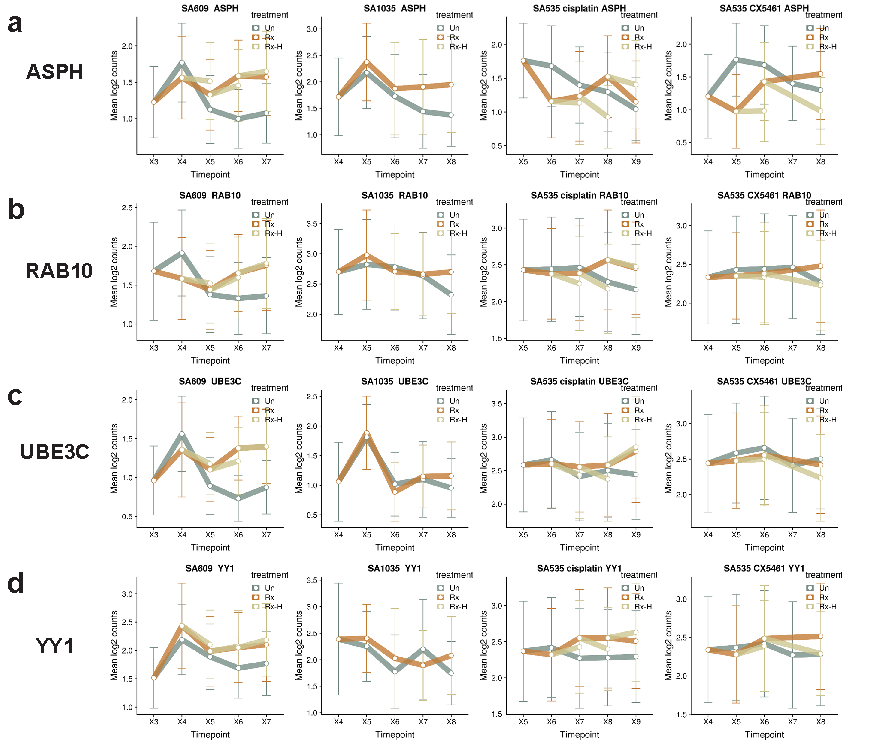
\includegraphics[width=\textwidth]{Figures/commongenesfromvolcanoplots.pdf}
	
\caption[Proportion of \textit{in-cis} and \textit{in-trans} regulated gene expression in scRNAseq data]
	{\small
	\textbf{Proportion of \textit{cis} and \textit{trans} regulated gene expression in scRNAseq data.}
	   Horizontal axis shows differential expression between two selected clones from all the three PDX treated and un-treated timeseries. Vertical axis gives percentage presence of genes in-cis or in trans. red bars represent in-cis and blue bars represent in -trans regulated gene expression.
	   \textbf{(a)} ASPH
	    \textbf{(b)} RAB10.
	    \textbf{(b)} UBE3C.
	     \textbf{c)} YY1
	}
	\label{fig:commongenesfromvolcanoplots}
\end{figure}

%------------------------------------------------------------------------

In \textbf{SA535} TNBC PDX, both timeseries from two different drugs showed up with somewhat distinct set of regulated genes. Interestingly, the first upregulated gene,\textit{(incis\_IU)}, that caught our attention was on chromosome X, \textbf{XIST}\cite{salama2020xist,chen2017long, chen2019up}, in both independently treated different drug series \textbf{(\autoref{fig:Volcanotrackplots2.pdf} c, d right)}. 
In addition, other \textbf{cisplatin} related set of genes in this PDX comprised of \textbf{TACC1}, which is upregulated \textit{(incis\_IU)} on chromosome 8, known to be amplified in 10-15\% of human breast cancers and plays a role in interactions between centrosomes and microtubules \cite{ray2004genomic, gergely2000tacc, shakya2018high},
\textbf{COX17}, downregulated in or resistant clone, is a human copper chaperone, that binds cisplatin \cite{katano2002acquisition, zhao2014cisplatin}, \textbf{CYP27A1} is more specific in hapatocellular carcinome but also seem to be expressed in high grade breast tumors \cite{liang2019cyp27a1, wu201327}, \textbf{SLC31A2}, are membrane transporters known to be downregulated in resistance \cite{bai2017structural}. Other significant genes that could be under consideration for further validations in our cisplatin related data sets were \textbf{DST}  \cite{salerno2016human,lee2012differentially}, \textbf{HMGCS1} \cite{walsh2020mevalonate},
\textbf{TAGLN} \cite{wu2014transgelin, elsafadi2020transgelin},
\textbf{KRT16} \cite{huang2019novel},
\textbf{IFITM3} \cite{liu2019ifitm3} and
\textbf{S100A7} \cite{zhang2019clinical, mayama2018olfm}.

In \textbf{SA535} treated with \textbf{CX-5461}, the differential expression of resistant and sensitive clones also resulted in known cancers related genes but potential candidates to explore further in relation to CX-5461 resistance related mechanisms. Highlighting some more includes \textbf{MMP7}, which is correlated with cancer invasion, metastasis, and poor prognosis \cite{mcgowan2008matrix} ,
\textbf{TMEM45A}, known to cause chemoresistance in breast cancer \cite{schmit2019characterization},
\textbf{ETS2}, functions as an oncogene and plays a key role in the progression of hypopharyngeal cancer and associated with poor prognosis \cite{fu2017high, ge2008role}.
\textbf{COX7A2} is downregulated in resistant clone which is negatively correlated with prognosis \cite{deng2018overexpression},
\textbf{POLR2C} mutation is known to progress ovarian cancers and its found downregulated in our resistant clone \cite {moriwaki2017polr2c} and
\textbf{OLFM4} is reported to be highly expressed in cancers, including gastric cancer, colon cancer, and pancreatic cancer and to promote tumor progression by inducing cell cycle progression and enhancing tumor invasion and metastasis \cite{ashizawa2019olfm4}.

\subsubsection{Trend of genes common in all four TNBC PDX under chemotherapy}
We next asked whether there is drug induced adaptive expression of common genes that could be seen in all timeseries. 
 Few genes were enlisted that were found to be increasing monotonically in all 4 TNBC PDX series. We recorded their expression at each time under various experimental conditions in all timeseries. Some of common genes were ASPH, CDKN2, RAB10, RCAN1, SCARB2, PAPOLA, UBE3C and YY1. The representative line trajectories from \textbf{ASPH}, which is known to be upregulated in breast carcinoma, hepatic carcinoma, cervical cancer and ovarian cancer and contributes to enhancing cell migration  \cite{zheng2020diverse,li2018expression, hou2018recent, lin2019asph}, tend to rise under the drug in all series but less significantly in SA535 treated with cisplatin \textbf{\autoref{fig:commongenesfromvolcanoplots} a}. 
\textbf{RAB10,(Member RAS Oncogene Family)} is also found to be increasing monotonically with each cycle of drug in all 4 TNBC PDX \textbf{\autoref{fig:commongenesfromvolcanoplots} b}. It has been recently demonstrated to be aberrantly expressed in some of the cancers and show biological significance in tumor progression and prognosis,  especially, in hepatocellular carcinoma \cite{wang2017rab10, he2002identification, jiang2016mir}. 
Another gene, \textbf{UBE3C} also seem to establish high expression in all 4 PDXs but more significantly in SA609 and SA535, treated with cisplatin \textbf{\autoref{fig:commongenesfromvolcanoplots} c}. The role of aberrant expression of ubiquitin Protein ligase E3C (UBE3C) has not been widely studied in triple negative breast cancers but in ovarian cancer, gastric cancer, renal cell carcinome and melanoma, it is known to promote proliferation and invasion and inhibition of apoptosis by activating the β-catenin signaling possibly via degradation of AXIN1 \cite{xiong2019mir, pan2015ubiquitin, zhang2020ube3c}.
 Zinc-finger protein \textbf{Yin Yang 1 (YY1)}, In our data, YY1 expression remained high under the drug as compare to most of untreated timepoints \textbf{\autoref{fig:commongenesfromvolcanoplots} c}. YY1 generally overexpressed in breast cancer cells 
is uniformly highly over-expressed in a wide range of human cancers including human colon cancer tissue samples. It involves numerous genes involved in cell proliferation, cell cycle, survival and cellular metabolism.  \cite{wan2012yin, chinnappan2009transcription, meliala2020biological}. Literature indicates that YY1 possesses a great potential as a biomarker for many cancers and can serve as a therapeutic target to impede cancer progression or sensitize cancer cells to chemotherapies \cite{wan2012yin, chinnappan2009transcription, meliala2020biological, shi2015role}.

\subsubsection{Proportions of genes \textit{in cis} and \textit{in trans} from various database}
Next, we probed that what proportion of genes exist \textit{in cis} or \textit{in trans} in our data set from a catalogue of various databases.
Three database were selected, including COSMIC \cite{vogelstein2013cancer}, core cancer fitness \cite{behan2019prioritization} and cisplatin related genes curated from last 10 years literature \textbf{\autoref{tab:Cisplatinrelatedgenes}}.
First we pulled the reference genes from these database that were intersecting with our \ac{DE} data and calculated if they are regulated with the change in copy number or not.

 In  SA609 TNBC PDX, the mean number of \textit{in cis} genes was 1173.8 (segment positions, $\sigma$ = 494 \textit{in cis} genes, max= 1640, min=215), SA1035 presented with the lowest \textit{in cis} with
 mean value of 187.8 (segment positions, $\sigma$ = 51 \textit{in cis} genes, max=246, min=144). SA535 in cisplatin timeseries showed mean number of 1056.9 \textit{in cis} genes (segment positions, $\sigma$ = 624 , max=1900, min=116), whereas, SA535 in CX-5461 exhibit highest number of mean \textit{in cis} value of 1400.7 (segment positions, $\sigma$ = 481 \textit{in cis} genes, max=1884, min=739).
 
 Overall, our results remained consistent with the fact that the proportion of \textit{in trans} regulation of gene expression is higher than the \textit{in cis} in all the time series PDXs and from all the reference lists.   
 
 Interestingly, we noticed that SA535 TNBC in both treatment regimes, inferred highest rate of \textit{in cis} genes with 28\% maximum, whereas, SA1035 TNBC possessing the lowest rate of 2.4\% maximum. SA609 TNBC showed 12.8\% of its highest \textit{in cis} gene rate \textbf{\autoref{fig:fig3_In_cispercentage}}.


%------------------------------------------------------------------------
 \begin{figure}
\centering
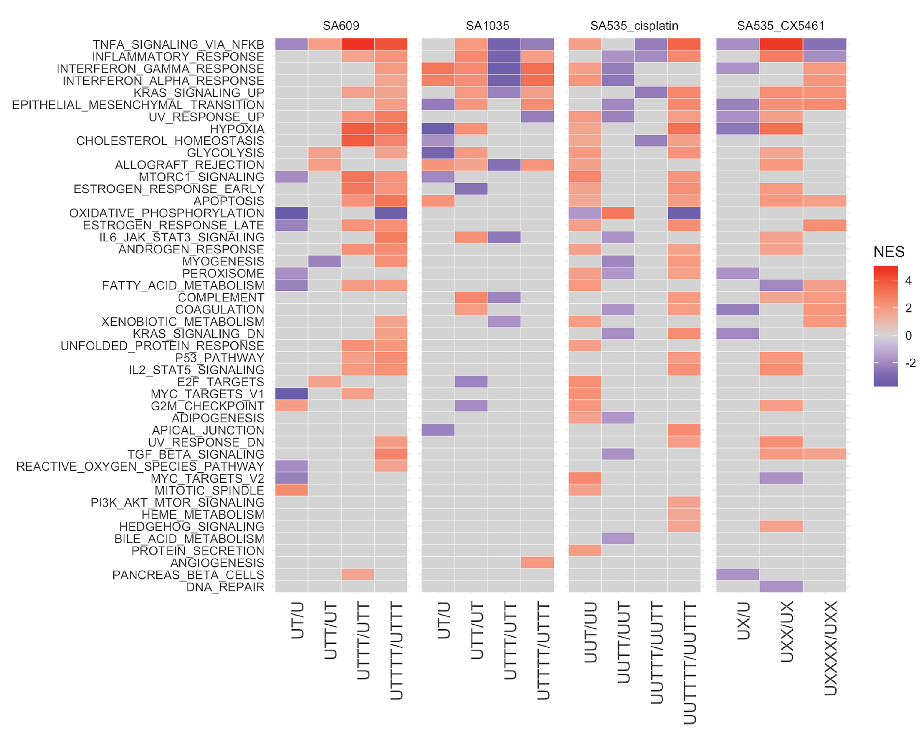
\includegraphics[width=\textwidth]{Figures/pathwaysevolution.pdf}
\caption[Summary of number of genes \textit{in-cis} and \textit{in-trans}]
	{\small
	\textbf{Pathways comparison over time under chemotherrapy in all PDX series}
	Vertical left column enlist the pathways analysed. Horizontal axis at the bottom, represents the comparisons made between the time points and the treatment status. each single `T' indicates the number of cycles of the treatment from cisplatin. Each `X' indicates number of cycles of CX-5461 treatment. Colour intensity identifies normalized enrichment score (NES). Horizontal axis on top denotes the IDs of TNBC PDX. A normalized enrichment score (NES) was calculated from a ranked gene set enrichment analysis (GSEA) \cite{shi2007gene} performed on each subset of differentially expressed genes using the hallmark gene set collection from MSigDB \cite{liberzon2015molecular}.  Significantly enriched pathways (adjusted p-value $<$ 0.01).
}
    \label{fig:pathwaysevolution}
    \end{figure}
%-------------------------------------------------------------------
\begin{figure}
\centering
  \includegraphics[width=\textwidth]{Figures/pathwaysnetwork.pdf}
\caption[Pathways enrichment analysis of PDX timeseries]
	{\small
	\textbf{Pathways enrichment analysis of PDX timeseries.}
	 	\textbf{(a)} Vertical axis on the left enlisting the pathways involved from a ranked gene set enrichment analysis (GSEA) \cite{shi2007gene}. Colour intensity identifies normalized enrichment score (NES). Horizontal axis on top denotes the IDs of TNBC PDX. \textbf{(b)} SA609 resistant vs sensitive clone.  A normalized enrichment score (NES) was calculated from GSEA, performed on each subset of differentially expressed genes using the hallmark gene set collection from MSigDB \cite{liberzon2015molecular}. Significantly enriched pathways (adjusted p-value $<$ 0.01). The grey to black coloured lines indicating the number of genes shared between pathways \textbf{(c)} same as \textbf{b} but SA1035 \textbf{(d)} same as \textbf{b} but SA535-cisplatin treated \textbf{(e)}same as \textbf{b} but SA535-CX-5461 treated
	}
	\label{fig:pathwaysnetwork}
\end{figure}

%-------------------------------------------------------------------
\subsection{Integrated transcriptome and pathway analyses revealed potential genes and key activated pathways in breast cancer}
Next, we generated a heatmap of pathway evolution from one treated time point to another in all timeseries TNBC PDX \textbf{\autoref{fig:pathwaysevolution}}. Most of the listed pathways were enriched at the later timepoints where tumor responses to the chemotherapies were comparatively less. 

\subsubsection{Profiling of signaling pathways reveals a distinct demarcation between SA1035 and rest of 3 TNBC PDX}
To assess the common pathways and their network connections, 
we profiled pathways enrichment scores between the resistant and sensitive clones of all TNBC PDX. 
Pathways specific differentially expressed genes were included in network enrichment analysis and the nodes were colored by NES value. Interestingly, SA1035 TNBC PDX demonstrated only three upregulated pathways in resistant versus sensitive clone, including oxidative phosphorylation (OXPHOS), Interferon alpha response \cite{provance2019deciphering} and interferon gamma response \cite{mojic2018dark} \textbf{\autoref{fig:pathwaysnetwork} a, second column}. \ac{OXPHOS} is known to be upregulated in cisplatin related drug resistance mechanism \cite{lee2017myc}. The later two pathways are not well studied in relation to tumor progression or drug resistance but there are some speculative research related to these interferons and cancer related immune mechanisms. In contrast to other TNBC PDX, SA1035 resistant clone also evinced downregulated pathways of hypoxia, TNFA signaling via NFKB, epithelial mesenchymal transition, MTORC1 signaling, KRAS signaling and apoptosis {\textbf{\autoref{fig:pathwaysnetwork} c}}.  
In addition to SA1035, only SA535 timeseries that was treated with CX-5461 showed interferons pathways upregulation. However, the rest of 3 TNBC PDX, SA609,SA535-cisplatin treated and SA535-CX5461 treated, showed commonly upregulated certain pathways, including, TNFA signaling via NFKB \cite{lagunas2008nuclear,ito2015down, ryan2019targeting}, hypoxia \cite{lee2012hypoxia, mcevoy2015identifying, deben2018hypoxia,li2019erk}, apoptosis, TGF Beta signaling \cite{zhang2019tgfbeta1} and Estrogen response \cite{zhu2018er}. E2F targets \cite{zheng2020upregulation} and G2M checkpoint \cite{visconti2016cell} were common between SA609 and SA535-CX5461 treated \textbf{\autoref{fig:pathwaysnetwork} a, first, third and fourth columns}. 

\subsubsection{Network inference reveals innovative connections in pathways of resistant clones} 
 The upregulated associated pathways in resistant versus sensitive clones, in \textbf{SA609 TNBC PDX}, comprised of TGF Beta signaling, Hypoxia, TNFA signaling via NFkB, Cholesterol homeostasis, peroxisome and apoptosis. In addition to these, G2M checkpoint and E2F targets were found to be upregulated with $>$40 common genes between these two pathways. Mitotic spindle pathway upregulation was also associated with sharing of $>$10 genes with E2F and G2M check point pathways \textbf{\autoref{fig:pathwaysnetwork} b}.





\textbf{\autoref{fig:pathwaysnetwork} b, c, d, e}. 

\subsubsection{Gene co-expression network analysis apprise biological processes relationship}
  

\subsubsection{Gene specific expression trajectories exemplified systematic response to sustained treatment}







%------------------------------------------------------------------------
\begin{figure}
\centering
  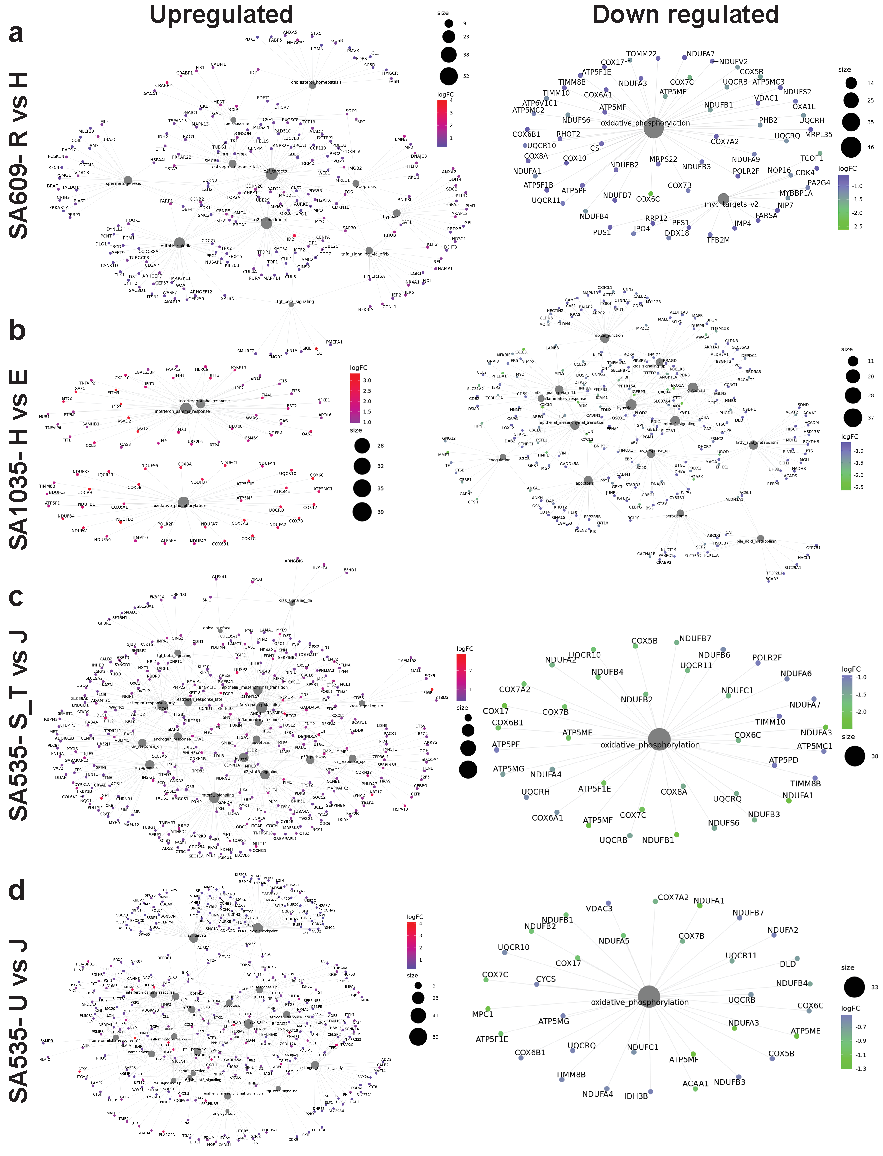
\includegraphics[width=\textwidth]{Figures/genenetworkanalysis.pdf}
\caption[DE of resistant and sensitive clonealign defined clones]
	{\small
	\textbf{Gene network analysis showing up-and downregulation resistant and sensitive clones across timeseries PDX.}
	\textbf{(a)} Normalized enrichment score of Pathways between resistant and sensitive clone of all treated timeseries PDXs.
	    \textbf{(b)} Pathway enrichment network comparison of clone }
		\label{fig:genenetworkanalysis}
\end{figure}

%-------------------------------------------------------------------

\begin{figure}
\centering
 \includegraphics[width=\textwidth]{Figures/generegressionanalysis.pdf}
	
\caption[Gene expression changes over time]
	{\small
	 \textbf{Gene expression changes over time in all 4 TNBC PDX timseries} .
	}
	\label{fig:generegressionanalysis}
\end{figure}



\section{Discussion}

By using clonealign, we were able to assign single cell RNAseq to  DLP+ clones and we observed similar clonal proportion. UMAP suggested that the clones are behaving in relatively monomorphic way. From global survey of the copy number driven change in expression, \textit{in cis} proportion was found to be less as compared to the \textit{in trans} which is consistent with the mutation effects on expression. We know that cis-regulatory mutations are skewed toward decreased expression while trans-regulatory mutations are skewed toward increased expression \cite{metzger2016contrasting}.

The magnitude of individual gene expression differences between resistant and sensitive clones showed modest range of \textit{in cis} and \textit{in trans}. Although most of the genes are different but there are pathways that were common among the TNBC PDX models. 

SA1035 TNBC PDX behaves a little different as compared to the other two PDX models based on the activated pathways and proportion of individual gene expression \textit{in cis} and \textit{in trans}. This could be possibly explained based on the initial heterogeneity of this tumor. The DLP+ heatmap showed less heterogeneity as compared to SA609 and SA535 and the later was found to show the most heterogeneous tumor.

Some of the gene clusters were found to be increasing or decreasing along the time series of the PDX models but they require further detailed investigation at individual gene level to get enough evidence.






%\subsubsection{SA609-TNBC-FBI PDX up regulated pathways in resistant clone}


%\subsubsection{SA535-TNBC-BRCA deficient PDX up regulated pathways in resistant clone}
%Next we compared the emerging clone under drug pressure with the clone that could not survive the repeated drug exposures. We identified the following significantly up regulated pathways:
%- Apoptosis, Epithelial mesenchymal transition, Hypoxia, mitotic spindle, MTORC1 signaling, MYC targets-V1, P53 pathway, TGF Beta signaling, TNFA signalling via NFKB, UV response up, UV response down, KRAS signaling, Angiogenesis, PI3K AKT MTOR signaling, unfolded protein response.


%\subsubsection{SA1035-TNBC-APOBEC deficient PDX up regulated pathways in resistant clone}




%\subsection{key Pathways and genes shared among the three TNBC PDX}




%\subsection{Distinct genes monotonically increasing and decreasing with drug} 


